% =====================================================================
%  Fig. 2 -- Patch-Graph Construction Module (single-column width)
% =====================================================================
\documentclass[tikz,border=3pt]{standalone}
\usepackage{helvet}
\renewcommand{\familydefault}{\sfdefault}
\usepackage{amsmath,amssymb}
\usetikzlibrary{arrows.meta,positioning,calc,fit,backgrounds,decorations.pathreplacing}

\hyphenpenalty=10000 \exhyphenpenalty=10000 \pretolerance=10000 \tolerance=9999

\definecolor{cGraph}{HTML}{5B4B8A}  \definecolor{cGraphBg}{HTML}{ECE8F6}
\definecolor{cTrain}{HTML}{2A9D8F}  \definecolor{cTrainBg}{HTML}{DEF2EF}
\definecolor{cFuse}{HTML}{9E2A2B}
\definecolor{cInk}{HTML}{1F2933}
\definecolor{dInt}{HTML}{4C3D7A}
\definecolor{dEdg}{HTML}{8E7FBF}
\definecolor{dCor}{HTML}{C9BFE4}

\begin{document}
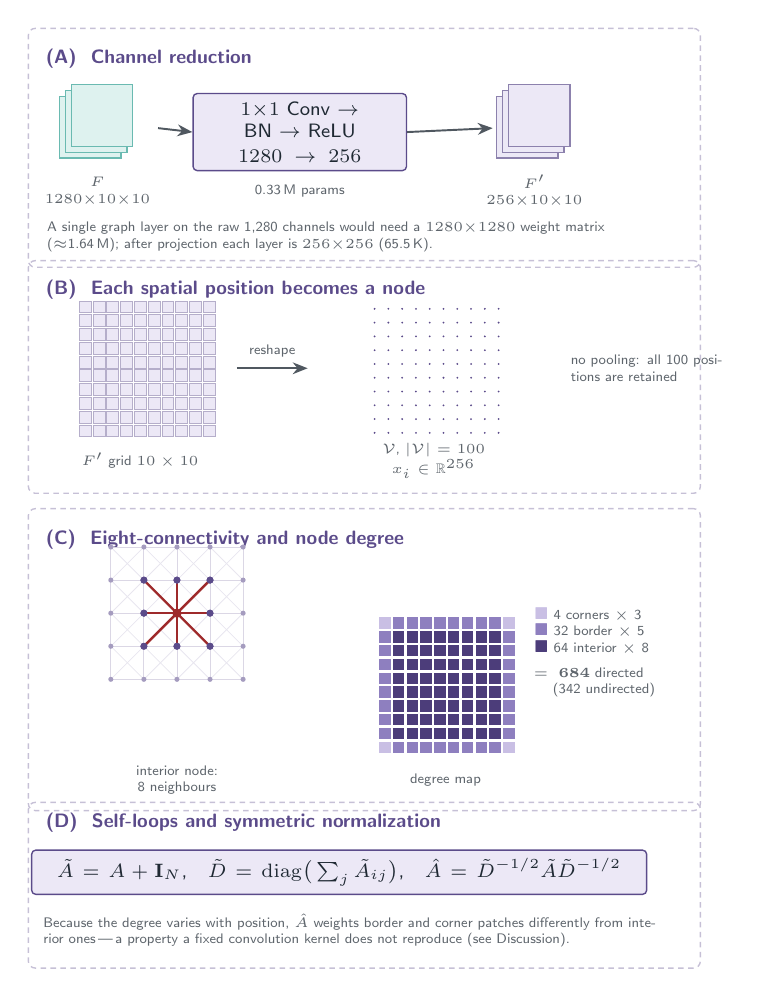
\begin{tikzpicture}[
  font=\scriptsize,
  blk/.style 2 args={draw=#1, fill=#2, rounded corners=1.5pt, line width=.5pt,
                     align=center, text=cInk, inner sep=3pt},
  flow/.style={-{Stealth[length=1.9mm,width=1.5mm]}, line width=.7pt, draw=cInk!78},
  shp/.style={font=\tiny, text=cInk!72, inner sep=1pt},
  ttl/.style={font=\scriptsize\bfseries, text=cGraph},
  panel/.style={draw=cGraph!35, rounded corners=2.5pt, line width=.5pt,
                dash pattern=on 2pt off 1.6pt},
]

% ================= PANEL A : channel reduction =================
\node[ttl, anchor=west] at (0,10.88) {(A)\ \ Channel reduction};

\foreach \i in {0,1,2}{
  \draw[draw=cTrain!70, fill=cTrainBg, line width=.45pt]
    (0.30+\i*0.075, 9.62+\i*0.075) rectangle ++(0.78,0.78);}
\node[shp, align=center] at (0.78,9.20) {$F$\\ $1280{\times}10{\times}10$};

\node[blk={cGraph}{cGraphBg}, text width=25mm] (proj) at (3.35,9.95)
  {$1{\times}1$ Conv $\rightarrow$ BN $\rightarrow$ ReLU\\[1pt] $1280 \rightarrow 256$};
\node[shp, align=center] at (3.35,9.20) {0.33\,M params};

\foreach \i in {0,1,2}{
  \draw[draw=cGraph!70, fill=cGraphBg, line width=.45pt]
    (5.85+\i*0.075, 9.62+\i*0.075) rectangle ++(0.78,0.78);}
\node[shp, align=center] at (6.33,9.20) {$F'$\\ $256{\times}10{\times}10$};

\draw[flow] (1.55,10.00) -- (proj.west);
\draw[flow] (proj.east) -- (5.80,10.00);

\node[shp, anchor=west, text width=76mm, align=left] at (0.10,8.62)
  {A single graph layer on the raw 1{,}280 channels would need a
   $1280{\times}1280$ weight matrix ($\approx$1.64\,M);
   after projection each layer is $256{\times}256$ (65.5\,K).};

% ================= PANEL B : positions -> nodes =================
\node[ttl, anchor=west] at (0,7.95) {(B)\ \ Each spatial position becomes a node};

\begin{scope}[shift={(0.55,6.08)}, scale=.175]
  \foreach \x in {0,...,9}\foreach \y in {0,...,9}{
    \draw[draw=cGraph!45, fill=cGraphBg, line width=.28pt]
      (\x,\y) rectangle ++(0.86,0.86);}
\end{scope}
\node[shp, align=center] at (1.32,5.78) {$F'$ grid $10\times10$};

\draw[flow] (2.55,6.95) -- (3.45,6.95);
\node[shp, anchor=south] at (3.00,7.05) {reshape};

\begin{scope}[shift={(4.30,6.13)}, scale=.175]
  \foreach \x in {0,...,9}\foreach \y in {0,...,9}{
    \fill[cGraph] (\x*1.0,\y*1.0) circle (2.1pt);}
\end{scope}
\node[shp, align=center] at (5.05,5.78)
  {$\mathcal{V}$, $|\mathcal{V}|=100$\\ $x_i \in \mathbb{R}^{256}$};

\node[shp, anchor=west, text width=20mm, align=left] at (6.75,6.95)
  {no pooling: all 100 positions are retained};

% ================= PANEL C : connectivity + degree =================
\node[ttl, anchor=west] at (0,4.78) {(C)\ \ Eight-connectivity and node degree};

% -- 5x5 neighbourhood zoom
\begin{scope}[shift={(0.95,3.00)}, scale=.42]
  \foreach \x in {0,...,4}\foreach \y in {0,...,4}{\coordinate (m\x\y) at (\x,\y);}
  \foreach \x in {0,...,4}\foreach \y in {0,...,3}{
    \draw[cGraph!22, line width=.3pt] (m\x\y) -- (m\x\the\numexpr\y+1\relax);}
  \foreach \x in {0,...,3}\foreach \y in {0,...,4}{
    \draw[cGraph!22, line width=.3pt] (m\x\y) -- (m\the\numexpr\x+1\relax\y);}
  \foreach \x in {0,...,3}\foreach \y in {0,...,3}{
    \draw[cGraph!14, line width=.28pt] (m\x\y) -- (m\the\numexpr\x+1\relax\the\numexpr\y+1\relax);
    \draw[cGraph!14, line width=.28pt] (m\x\the\numexpr\y+1\relax) -- (m\the\numexpr\x+1\relax\y);}
  % highlighted 8-neighbourhood of the centre node
  \foreach \dx/\dy in {-1/-1,-1/0,-1/1,0/-1,0/1,1/-1,1/0,1/1}{
    \draw[cFuse, line width=.85pt]
      (2,2) -- ($(2,2)+(\dx,\dy)$);}
  \foreach \dx/\dy in {-1/-1,-1/0,-1/1,0/-1,0/1,1/-1,1/0,1/1}{
    \fill[cGraph] ($(2,2)+(\dx,\dy)$) circle (3.0pt);}
  \foreach \x in {0,...,4}\foreach \y in {0,...,4}{\fill[cGraph!55] (m\x\y) circle (2.2pt);}
  \foreach \dx/\dy in {-1/-1,-1/0,-1/1,0/-1,0/1,1/-1,1/0,1/1}{
    \fill[cGraph] ($(2,2)+(\dx,\dy)$) circle (3.0pt);}
  \fill[cFuse] (2,2) circle (4.0pt);
\end{scope}
\node[shp, align=center] at (1.79,1.72) {interior node:\\ 8 neighbours};

% -- degree map
\begin{scope}[shift={(4.35,2.06)}, scale=.175]
  \foreach \x in {1,...,8}\foreach \y in {1,...,8}{
    \draw[draw=white, fill=dInt, line width=.3pt] (\x,\y) rectangle ++(0.9,0.9);}
  \foreach \x in {1,...,8}{
    \draw[draw=white, fill=dEdg, line width=.3pt] (\x,0) rectangle ++(0.9,0.9);
    \draw[draw=white, fill=dEdg, line width=.3pt] (\x,9) rectangle ++(0.9,0.9);
    \draw[draw=white, fill=dEdg, line width=.3pt] (0,\x) rectangle ++(0.9,0.9);
    \draw[draw=white, fill=dEdg, line width=.3pt] (9,\x) rectangle ++(0.9,0.9);}
  \foreach \x/\y in {0/0, 0/9, 9/0, 9/9}{
    \draw[draw=white, fill=dCor, line width=.3pt] (\x,\y) rectangle ++(0.9,0.9);}
\end{scope}
\node[shp, align=center] at (5.20,1.72) {degree map};

% -- degree legend / edge accounting
\node[shp, anchor=north west, text width=22mm, align=left] at (6.28,3.95)
  {\textcolor{dCor}{$\blacksquare$}\ 4 corners $\times$ 3\\
   \textcolor{dEdg}{$\blacksquare$}\ 32 border $\times$ 5\\
   \textcolor{dInt}{$\blacksquare$}\ 64 interior $\times$ 8\\[3pt]
   $=\ \mathbf{684}$ directed\\ \phantom{$=$}\ (342 undirected)};

% ================= PANEL D : normalization =================
\node[ttl, anchor=west] at (0,1.18) {(D)\ \ Self-loops and symmetric normalization};

\node[blk={cGraph}{cGraphBg}, text width=76mm] (norm) at (3.85,0.55)
  {$\tilde{A}=A+\mathbf{I}_{N}$,\quad
   $\tilde{D}=\mathrm{diag}\big(\textstyle\sum_{j}\tilde{A}_{ij}\big)$,\quad
   $\hat{A}=\tilde{D}^{-1/2}\tilde{A}\tilde{D}^{-1/2}$};

\node[shp, anchor=north west, text width=78mm, align=left] at (0.05,0.06)
  {Because the degree varies with position, $\hat{A}$ weights border and corner
   patches differently from interior ones\,---\,a property a fixed convolution
   kernel does not reproduce (see Discussion).};

\begin{scope}[on background layer]
  \node[panel, fit={(0.02,8.35) (8.32,11.15)}] {};
  \node[panel, fit={(0.02,5.48) (8.32,8.20)}] {};
  \node[panel, fit={(0.02,1.45) (8.32,5.05)}] {};
  \node[panel, fit={(0.02,-0.55) (8.32,1.32)}] {};
\end{scope}

\end{tikzpicture}
\end{document}
